\documentclass{scrbook} % <= Druckversion: "scrbook", Bildschirmversion: "scrreprt"
\newcommand\bcor{8mm} % <= falls nötig, Bindungskorrektur für Druckversion (ohne Layoutzerstörung bei Anpassung)
\usepackage{osm-thesis}
\usepackage{listings}

% ABOUT
\newcommand{\hpitype}{Master Thesis}
\newcommand{\hpiauthor}{Florian Rösler}
\newcommand{\hpititle}{Dynamic OpenCL - Distributed Computing on Cloud Scale}
\newcommand{\hpititleother}{Dynamic OpenCL - Verteiltes Rechnen für Rechenzentren mit angebundenen Clouds} % <= das Studienreferat verlangt einen deutschen UND englischen Titel
\newcommand{\hpisupervisor}{Prof.\,Dr.\,Andreas Polze, Max Plauth}
\newcommand{\hpichair}{Fachgebiet für Betriebssysteme und Middleware}
\newcommand{\hpiexternalsupervisor}{}
\newcommand{\hpiexternal}{}
\newcommand{\hpidate}{\today}

% DOCUMENT
%\KOMAoption{draft}{true} % <= z.B. zum "Debuggen" der Overfull-Boxes
\bibliography{bibliography}

\begin{document}
	\selectlanguage{english}

	% Einband
	\pagenumbering{alph}
	\ifisbook\begin{titlepage}
	\setlength{\evensidemargin}{0.5\evensidemargin+0.5\oddsidemargin}
	\setlength{\oddsidemargin}{\evensidemargin}

	\centering

	\raisebox{-0.5\height}{
\includegraphics[width=5.5cm]{images/hpi_logo_black.pdf}}
	\hspace*{.2\textwidth}
	\raisebox{-0.5\height}{
\includegraphics[width=4cm]{images/uni_logo_black.pdf}}
	

	\vspace*{4\baselineskip}
	{\usekomafont{subject}\hpitype}\par
	\vspace*{2\baselineskip}
	{\usekomafont{title}\hpititle\par}
	\vspace*{\baselineskip}
	{\usekomafont{subtitle}\hpititleother}\par
	\vspace*{2\baselineskip}
	{\usekomafont{author}\hpiauthor}\par
	
	\vfill
	
	{\usekomafont{date}Hasso-Plattner-Institut an der Universität Potsdam}\par
	\vspace*{\baselineskip}
	{\usekomafont{date}\hpidate}\par
	
\end{titlepage}\fi
	\ifisbook\cleardoubleemptypage\fi

	% (Haupt-)Titelseite, Abstract, ggf. Danksagung & Inhaltsverzeichnis
	\pagenumbering{roman}
	\begin{titlepage}
	\centering

	\raisebox{-0.5\height}{
\includegraphics[width=5.5cm]{images/hpi_logo_srgb.pdf}}
	\hspace*{.2\textwidth}
	\raisebox{-0.5\height}{
\includegraphics[width=4cm]{images/uni_logo_srgb.pdf}}

	\vspace*{4\baselineskip}
	{\usekomafont{subject}\hpitype}\par
	\vspace*{2\baselineskip}
	{\usekomafont{title}\hpititle\par}
	\vspace*{\baselineskip}
	{\usekomafont{subtitle}\hpititleother}\par
	\vspace*{2\baselineskip}
	{\usekomafont{author}\hpiauthor}\par

	\vfill
	{\textbf{Betreuung}\\\usekomafont{publishers}\hpisupervisor\\\textit{\hpichair}\\\smallskip\textbf{\normalfont\hpiexternalsupervisor}\\\textit{\hpiexternal}}

	\vspace*{2\baselineskip}
	{\usekomafont{date}Hasso-Plattner-Institut an der Universität Potsdam}\par
	\vspace*{\baselineskip}
	{\usekomafont{date}\hpidate}\par

	\setcounter{page}{1}

\end{titlepage}


	\ifisbook\cleardoubleemptypage\fi\begin{center}\textsf{\textbf{Abstract}}\end{center}

\noindent Creating parallelized software in order to reduce execution times is one of the main challenges in computer science. Writing parallel programs requires programmers to obtain extensive low level knowledge about the hardware specifications and the standards of the corresponding programming models. When enhancing multi-core programs to harness multiple machines of a cluster, another layer of indirection is added, hence significantly increasing code complexity. The goal of this research is to create a parallel computation framework that allows to distribute workloads among central processing units and graphics processing units within a cluster without deep knowledge of the underlying technologies. Thus, the framework is expected to provide a high level application programming interface that should be usable by novice programmers. Additionally it should be possible to adjust computational resources dynamically depending on changing cluster utilizations.

Various parallelization methods, such as OpenMP, Message Passing Interface and OpenCL, are illustrated and discussed regarding their ability to contribute to the framework. Because of the possibility to produce portable code following a fixed programming model, OpenCL is chosen as the underlying base technology. In combination with dOpenCL, OpenCL programs can be executed on remote machines via network without changes to the original code. The resulting parallelization potential of OpenCL in conjunction with dOpenCL is abstracted behind the main contribution of this research -- Dynamic OpenCL. Dynamic OpenCL is written in Java and allows programmers to create distributed OpenCL programs in Java by employing Aparapi for code translations. It contains sophisticated mechanisms for cluster management and dynamic resource adjustments that enable its operation in various cluster setups such as hybrid clusters that are comprised of local and cloud resources. Depending on the respective cluster environment it is possible to adjust scheduling algorithms in order to gain performance improvements.

During an extensive evaluation it is shown that the framework can introduce significant performance benefits by distributing selected tasks with almost linear speedups. Even in heavily network-bound cluster setups that incorporate cloud resources, Dynamic OpenCL is able to increase performance noticeably by providing a network-aware scheduling mechanism. Based on Dynamic OpenCL a prototypical web server is built that allows users to submit computations through a user interface and enables them to decrease execution times by booking additional cloud resources.

It is concluded that Dynamic OpenCL is able to provide speedups in various cluster environments, mainly depending on the nature of submitted workloads and available network bandwidths to remote devices. With further improvements that aim at reducing the impact of limited network bandwidths, the speedup potential might be increased even further in the future.

% <= Wenn die Arbeit auf Englisch verfasst wurde, verlangt das Studienreferat einen englischen UND deutschen Abstract

%\vspace{2cm}
%\selectlanguage{english}
%\begin{center}\textsf{\textbf{Abstract}}\end{center}
%Lorem ipsum dolor sit amet, consetetur sadipscing elitr, sed diam nonumy eirmod tempor invidunt ut labore et dolore magna aliquyam erat, sed diam voluptua. At vero eos et accusam et justo duo dolores et ea rebum. Stet clita kasd gubergren, no sea takimata sanctus est Lorem ipsum dolor sit amet. Lorem ipsum dolor sit amet, consetetur sadipscing elitr, sed diam nonumy eirmod tempor invidunt ut labore et dolore magna aliquyam erat, sed diam voluptua. At vero eos et accusam et justo duo dolores et ea rebum. Stet clita kasd gubergren, no sea takimata sanctus est Lorem ipsum dolor sit amet.
%\selectlanguage{ngerman}


	\tableofcontents
	\cleardoublepage

	% Textteil
	\pagenumbering{arabic}
  \chapter{Introduction}

\section{Motivation}

At the current state of technology, computers with multiple compute processing units (abbr. CPU) cores are common and even small devices like smartphones are usually manufactured with a multi-core architecture. Programs that want to harness the full potential of a multi-core computer have to be constructed accordingly.

Additionally, certain use cases require more computational power than a single machine can provide. Therefore it is mandatory to connect multiple machines to collectively solve a problem. For example researchers recently created a method to break a widely used cryptographic hash function that requires resources equivalent to more than 6500 CPU years to compute \cite{shattered}. A single machine at the current level of technology would therefore require too long in order to deliver the desired results. At the same time certain physical factors are limiting further quick advancements concerning CPU speeds \cite{end_of_moores_law}\cite{end_of_silicon} so that many problems will still require multiple machines in the future for time efficient computations.

As of today, there are various available approaches for programmers to distribute workloads across multiple cores of a single machine or among multiple machines grouped as a cluster. Enhancing single threaded code to a multithreaded program that runs on multiple machines in parallel adds several layers of complexity to a project, which may introduce errors and increased maintenance efforts.

Frameworks like Open Multi-Processing (abbrv. OpenMP), CUDA or Open Computing Language (abbr. OpenCL) allow for the parallel utilization of resources within a machine but in return require programmers to learn extensive APIs or write code in low level languages like C.
At the same time cluster distribution approaches like Hadoop MapReduce require extended configuration management of the participating nodes. MapReduce as well as other techniques like the Message Passing Interface (abbrv. MPI) also add a layer of complexity to the written program code that is entirely focused on synchronizing the distributed parts.
Ultimately, the combination of both levels of parallelization may lead to additional problems, which distract programmers from focusing on the underlying algorithm.

While the creation of distributed algorithms implicates various problems on its own, running these programs in a cost efficient manner represents another elaborate task. Clusters dedicated to running computations in a shared environment should have as little underutilization as possible in order to minimize costs. Therefore the dynamic adaption of resources to the actual performance requirements is a challenge with significant monetary benefits. As a result, cloud services have seen a steady increase in revenue due to their flexible billing options that allow booking resources for short amounts of time \cite{gartner_2017}. Still, a pure cloud approach may introduce several disadvantages like higher costs or reduced performance due to geographical distances between the user and the utilized resources. Accordingly, a hybrid approach appears beneficial, providing a steady baseline of performance with local hardware. In the case of computational peaks additional resources might be booked from an external provider, which allows for lower costs and better quality of service during times with high resource demands.

While there are existing solutions to run distributed code most usable frameworks do not offer programmers to distribute their workloads among varying cluster configurations at a high abstraction level. Therefore the goal of this research is to create a framework that combines present partial solutions and provides additional functionality.

\section{Goals}
\label{goals}
The main goal of this research is to provide a framework that assists programmers to distribute their programs within a hybrid cluster. Thus, the following requirements are defined in order to streamline the development:

\begin{description}[style=nextline]
    \item [Heterogeneity]
    The framework should support modern CPUs and GPUs. Thus, devices by the following vendors should be included: AMD, ARM, Intel and NVIDIA. Therefore various workloads and their specific hardware demands can be supported. Additionally, heterogeneous hardware allows for a more granular employment of the required resources. For example a more cost saving ARM CPU could be utilized in low demand situations instead of a more potent but also energy demanding Intel CPU.

    \item [Resource Scalability]
    For isolated workloads the required computational power may be estimated accordingly to determine the appropriate resources. As soon as an infrastructure is provided to multiple users that can submit computations it becomes challenging to reach a steady utilization of the cluster. Thus providing static resources to a fluctuating amount of incoming computations likely leads to periods of underutilization or congestions. Therefore it is desirable to have the ability to dynamically increase the computational power of the cluster. One way to achieve this is the utilization of external cloud services like Microsoft Azure, Amazon EC2 etc.

    \item [Scalable Speed]
    While the general size of a cluster should be adjustable for overall resource utilization the allocation of resources to a specific task also has to be considered. It is desirable that the user is able to scale the execution speed of their respective workloads as real-world deadlines could put boundaries on the amount of available time for a computation to finish. Therefore it must be possible dynamically adjust resources for a workload without interrupting the overall execution. With that ability the framework would be enabled to handle burst scenarios as well as save resources in the case of continuous low computational demand by a computation.

    \item [Ease of Programming]
    The introduced framework should provide programmers with an easy to use distribution mechanism without adding noticeable overhead to their development process. Preferably the resulting code should be created in a modern high level language on a high abstraction level.

    \item [Workload Diversity]
    While the submitted workloads could differ in size and required resources they might also have different hardware requirements. For instance, several workloads within the system could be optimized for CPUs and others for GPUs. The framework should support the execution of these workload types and additionally optimize the distribution across available hardware from a global system view.

    \item [Optimized Scheduling]
    Aside from various hardware that workloads can be optimized for, running programs on a hybrid cloud adds the issue of networking distances between the local cluster and the external cloud. Thus, certain tasks may see performance improvements when run locally instead of being initially sent to external resources. It is desirable to take these factors into account and consider network distances and bottlenecks during scheduling decisions.

\end{description}

  \chapter{Basics}

\section{Distribution Methods}

\subsection{OpenMP}
OpenMP represents a compiler extension that allows programmers to harness parallel computational power on a machine. It adds functions and flags to the respective language (C, C++ and Fortran are currently supported), which indicate the execution environment how to parallelize the program.

\subsection{MPI}
Although OpenMP is a very powerful tool for parallelization on a single machine, in order to write larger scale software, communications across multiple machines are necessary. One standard tool to achieve this is MPI.
MPI offers bindings to many languages and extends such by functions to identify a process and send as well as receive messages.

\subsection{MapReduce}
Due to its simple programming model, which mainly consists of a Map and a Reduce phase (there are many other phases in its implementations) it is a favoured approach for large clusters. Its most prominent implementation is Hadoop MapReduce, which in combination with Hadoop Distributed File System, is especially applicable for data intense jobs like log analysis and more.

\section{CUDA}

What is CUDA and what is it good for.

\section{OpenCL}

What is OpenCL and how does it differ from CUDA. Explain why it is not slower even though the general public thinks so.

\section{Aparapi}

Explain Aparapi's architecture and results.



  \chapter{Related Work}
\label{related}
In this chapter, several related research papers are explained that provide solutions to distribute computations for parallel execution. The first section covers OpenCL based approaches for parallelizing workloads on a single machine. The second section exhibits cluster distribution approaches based on OpenCL and CUDA.

\section{OpenCL Single Machine Distribution}

\subsection*{SOCL}
SOCL is an OpenCL based framework by \citeauthor{socl} that offers the following key features\cite{socl}:
\begin{itemize}
    \item Scheduling and load balancing of OpenCL kernels across multiple devices
    \item Management of memory transfers and coherency
    \item Dynamic adaption of kernel granularity
\end{itemize}

SOCL acts as a middleware with its own OpenCL ICD utilizing other installed ICDs on a machine. Thus, it is able to implement functionalities such as shared command queues for multiple devices by hiding the divided command queues of each device behind its API. Through this method load balancing techniques can also be applied.

One of the main features is the automatic granularity adaption of kernels, which allows the appropriate partitioning of tasks according to respective performance capabilities of devices in a heterogeneous cluster. To enable the adaption, programmers have to supply the framework with a function that indicates how to divide the kernel with its corresponding data.

\subsection*{Static multi-device load balancing for OpenCL}
\citeauthor{delalama_2012} published an approach for executing a single kernel on multiple devices as well as a load balancing mechanism based on each device's computing capabilities\cite{delalama_2012}.

Instead of splitting the data into smaller parts, they replicate its entirety across the utilized devices and merge the resulting output buffers. The merge process is based on an algorithm that finds buffer elements that underwent write operations during the execution and therefore should be present in the final result.


\subsection*{STEPOCL}

\citeauthor{stepocl} present a framework called STEPOCL, which offers programming multi-device applications using a specifically developed domain specific language\cite{stepocl}. Their promoted features are linear performance scaling with increasing device count as well as comparable performance to manually written OpenCL applications.

For a successful distribution of a Kernel across multiple devices STEPOCL requires OpenCL kernels to be submitted with an accompanying configuration that describes the following facts:
\begin{itemize}
    \item The data layout, which is used to split the data into subdivisions.
    \item A tiling configuration depending on the targeted device types. E.g. specific work-group sizes for CPUs and GPUs.
    \item A meta control flow of the application, which for example allows iterative algorithms.
\end{itemize}

Utilizing the configuration, an OpenCL Kernel is transformed to a new OpenCL Kernel that supports computing the partitioned data. During this compilation step STEPOCL identifies available devices that it can distribute the submitted workloads to. The distribution ratio of workloads per device is determined dynamically through a profiling mechanism that takes into account the performance of each device during the previous iteration of a Kernel execution. Therefore it is especially meaningful for iterative algorithms like n-body or k-means.

\subsection*{Fluidic Kernels}

The paper by \citeauthor{fluidic} proposes parallelizing kernels among the CPU and GPU of a machine\cite{fluidic}. They showcase two workloads that benefit rather from either CPU or GPU. In order to execute a Kernel in parallel on both devices, it is launched on the CPU as well as the GPU. While the GPU processes the submitted work-groups from the front, the CPU starts execution from the other end in so-called subkernels. After each finished subkernel, the CPU reports to the GPU the current work-group ID. During execution of each group, the GPU checks whether the current work-group has been processed yet and can therefore identify when it has reached work-groups that have already been computed by the CPU. Due to this mechanism, the overall task is distributed according to the computational capabilities of the participating devices.


\section{OpenCL and CUDA Cluster Distribution}
\label{cluster_distribution}
\subsection*{dOpenCL}

dOpenCL wraps the local OpenCL implementation in their own provided ICD. When the driver is used on the host, it forwards the API calls to specified machines in the network, which run a dOpenCL daemon\cite{dopencl}. The calls are received by the daemon and executed using the available OpenCL installation on the remote machine with the results being returned via network. This allows utilizing remote devices as if they were installed locally in the host machine. For example, a remote GPU would appear as if it was installed in the local machine's peripheral component interconnect express (abbr. PCIe) slot. Therefore OpenCL kernels do not require changes to run remotely as dOpenCL hides network transfers behind the standard OpenCL API. An overview of the architecture for an example cluster is shown in figure \ref{img:dopencl_arch}.

\begin{figure}[H]

	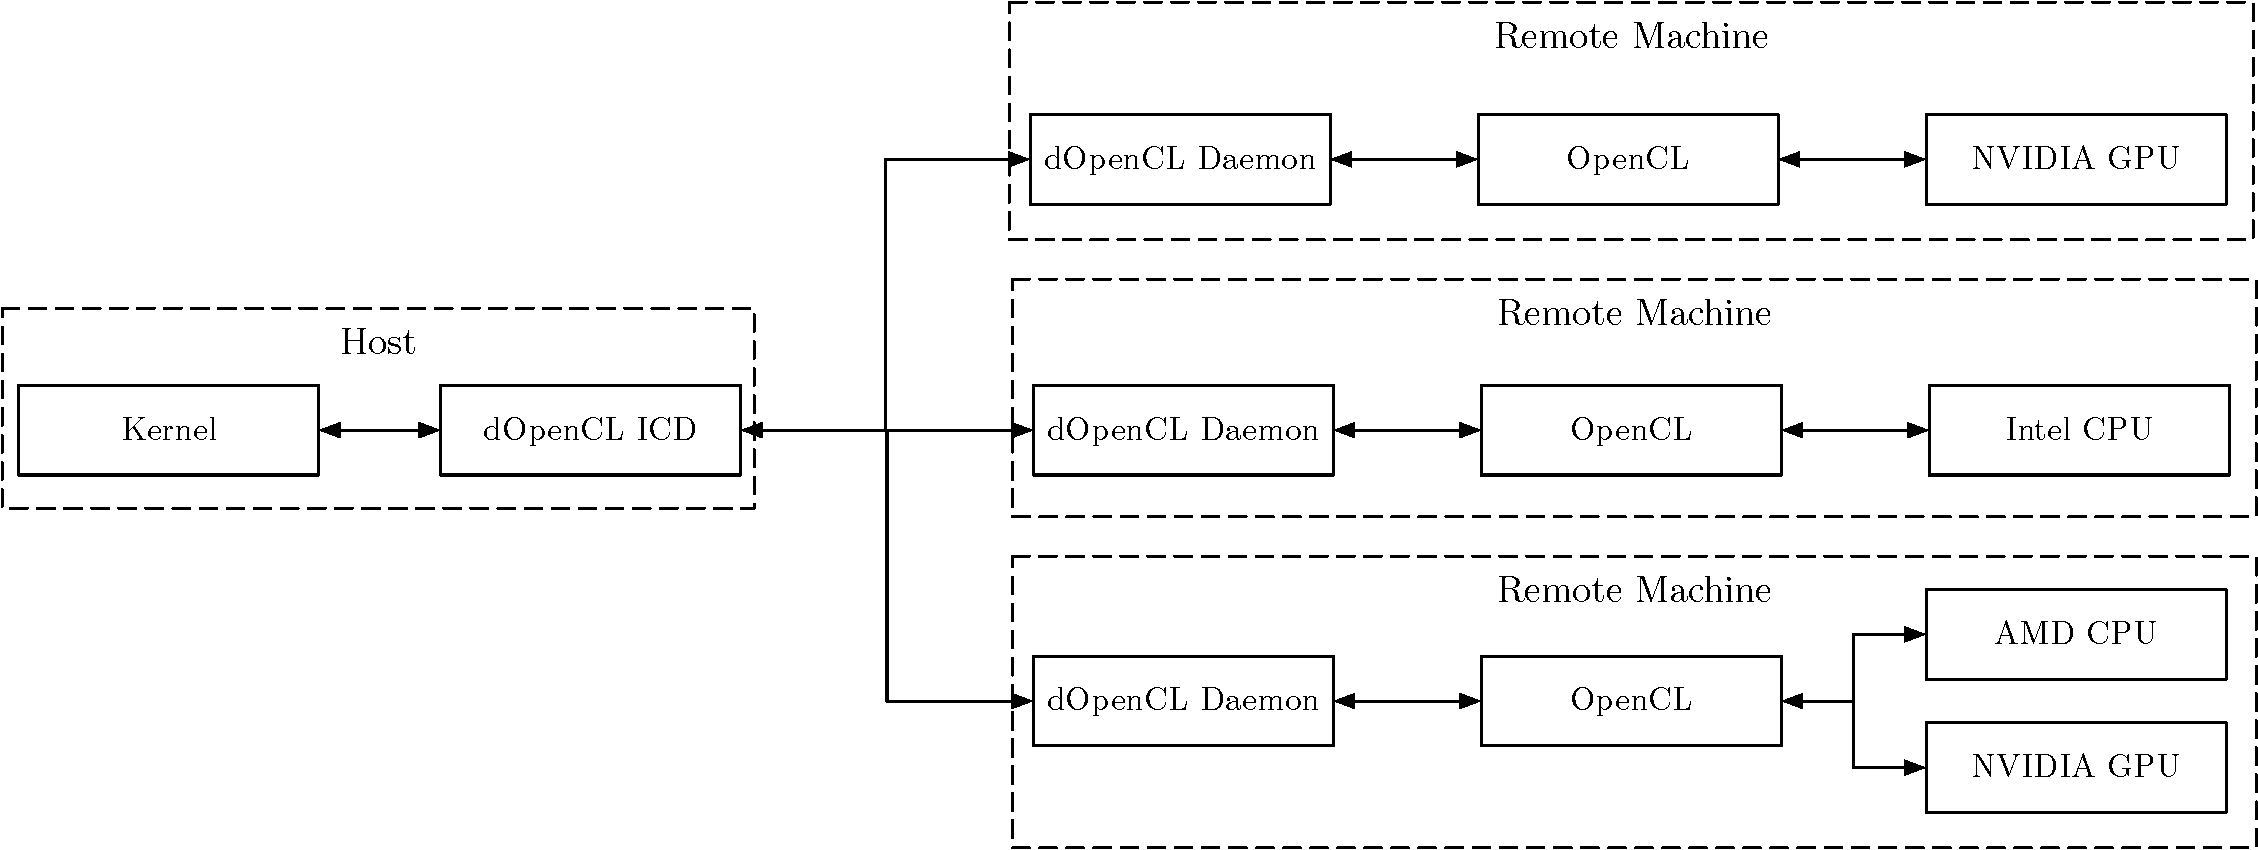
\includegraphics[width=0.95\textwidth]{drawings/dopencl_arch.pdf}
	\centering
	\caption{dOpenCL Architecture Overview}
	\label{img:dopencl_arch}
\end{figure}

dOpenCL supports shared cluster environments in which multiple OpenCL programs run concurrently by employing a device manager. It processes the assignment of devices to specific kernels and keeps track of device utilization within the cluster. Thus it ensures that a device is only used by a single Kernel at each point in time.

In their evaluation, \citeauthor{dopencl} show that for workloads with little data dOpenCL performs and scales well. They also compare dOpenCL's ability to transfer data to and from remote devices using Gigabit Ethernet against PCIe bandwidths. In the results, they conclude that dOpenCL reads the data 4.5x slower and writes 50x slower than their measured PCIe connection.

\subsection*{VirtualCL}

VirtualCL similarly to dOpenCL forwards OpenCL API calls to remote machines within a cluster\cite{virtualcl}. Just as dOpenCL it wraps its own ICD around the calls and refers them to running daemons on the remote machines.

\citeauthor{virtualcl} evaluate various applications comparing the local versus remote runtimes via VirtualCL. They show that network bandwidth and latency are the main bottlenecks of their solution but that long and compute intense kernels with low data transfers perform well.

VirtualCL offers an extension, called SuperCL, which is aimed at reducing network transfers by allowing multiple kernels being submitted to a remote node for serial execution. When these kernels depend on each other, the results are not transferred back and forth but stored in temporary buffers. It also supports more complex use cases like alternating iterative kernels on the same data set.

\subsection*{SnuCL}

SnuCL represents another library, aside from dOpenCL and VirtualCL, that provides a mechanism to access compute devices of a cluster as if they were available locally in a single local machine\cite{snucl}. Instead of simply forwarding API calls to remote machines, SnuCL heavily transforms kernels depending on the available runtimes of a machine. For example, it translates OpenCL to CUDA when only the CUDA platform is provided by the machine. Additionally, it can transform OpenCL code to C, which is then executed within a thread for each core of a CPU.

Furthermore, SnuCL introduces a virtual global memory, in which buffers may be shared among devices. It manages the consistency among shared buffers and attempts to minimize copy operations throughout the execution in order to save bandwidth. This is achieved by translating the OpenCL code to C, which is then used to identify whether a buffer will be written during execution. Buffers that are not written can therefore remain on a device without the requirement to be copied back to the host.

\subsection*{DistCL}
DistCL aims at merging multiple GPUs as a single virtual OpenCL device\cite{distcl}. To achieve this it abstracts the devices by representing them as one unified device while handling Kernel distribution and data transfers transparently. In order to enable parallelization of a Kernel, DistCL automatically splits it into multiple kernels with their respective required data, called subranges. In order to know, which data belongs to a subrange, programmers have to supply a meta-function that determines a memory access pattern. Based on the given function, DistCL can only transfer relevant data to a device that executes a subrange.

\subsection*{MultiCL}

MultiCL is built on top of SnuCL and promises to schedule kernels appropriately among multiple heterogeneous devices in a cluster\cite{multicl}. They offer a round robin approach as well as an autofit mechanism. When queuing a Kernel, a flag can be attached to it, which labels the assumed execution type. The available flags comprise \textit{compute intense}, \textit{memory bound}, \textit{I/O bound} or \textit{iterative}.

Their scheduling mechanism is able to employ a static or a dynamic algorithm. In their static scheduling approach, they profile all available devices in regards to memory bandwidth and instruction throughput. Based on these measurements, the best fitting device is selected with respect to the Kernel flag. In their dynamic scheduling algorithm they apply different mechanisms depending on the flag:

\begin{description}[align=left,leftmargin=0cm]
\item [Iterative] Cache previous Kernel execution times to find best performing device
\item [Compute-intensive] Kernels are transformed to smaller minikernels that are profiled on every available device to receive a performance indicator
\item [I/O-intensive] Extended data caching and minimized transfer operations for distributed executions
\end{description}

\subsection*{rCUDA}

rCUDA aims to reduce the number of GPU accelerators in a cluster by sharing the accelerators across machines within the network\cite{rcuda}. Thus not every machine is required to have a GPU installed. The applied technique comprises API forwarding to execute CUDA commands on the remote server and retrieve the respective result.

The main focus of the presented evaluation lies on power savings. When reducing the number of accelerators in a considered cluster by 90\%, a 20\% decrease in power consumption could be determined. Still, the authors are aware that this reduction can lead to a significant performance degradation depending on the application requirements within the cluster.

\subsection*{Virtualizing CUDA Enabled GPGPUs on ARM Clusters}

\citeauthor{arm_virtual_cuda} present an architecture in which a cluster of low-powered ARM devices accesses powerful remote NVIDIA GPUs through a virtual interface\cite{arm_virtual_cuda}. Their approach is based on API forwarding but features the connection of a private cluster to machines that are located at a cloud provider. In their example cluster, they connect local ARM devices to GPUs that are provided by Amazon's cloud.


	\chapter{Dynamic OpenCL}

\section{Distribution Approach}
\label{distribution}
As portrayed in section \ref{distribution} and \ref{related} many viable options exist to distribute tasks among devices within a single machine as well as across a cluster. This section will explain the reasons for selecting the fitting approaches based on the goals declared in section \ref{goals}.

At first it is important to evaluate the options for running tasks on multiple devices within a single machine. While low level solutions like OpenMP or OpenACC are matured, they add considerable overhead to programming efforts. All communication and synchronization across multiple cores and devices has to be handled by the programmer, which adds introduces a layer of complexity through the utilization of directives. Thus, programmers have to be knowledgable and experiences in utilizing these directives for an efficient execution.

Instead OpenCL will be selected for the distribution of tasks within a single machine. While CUDA offers similar capabilities as OpenCL, it only supports NVIDIA GPUs and completely lacks CPU support. This contradicts with the proposed goal of a heterogenous environment in which devices of different types and vendors cooperate. OpenCL introduces a standardized form in which algorithms have to be designed following the defined memory model and work-item approach. Even though many synchronization and communication calls like data transfers are abstracted away from the programmer, significant low level knowledge is required for building algorithms in the framework. In order to create a more simplified approach, difficult issues for programmers should also be abstracted behind a meaningful API. The necessary steps for that are covered in section \ref{abstraction}.

Even though many solutions for distributing computational workloads among machines in a cluster, most require significant cluster management or programming efforts. Because OpenCL is selected as the underlying computational framework on the machines, the cluster distribution technology has to fit its capabilities.

Similar to OpenMP, MPI has matured over decades as a standard solution for low level communications between multiple machines. As such it has also been used frequently in conjunction with OpenCL and inspired frameworks to build upon this combination. Still, MPI remains a significant contributor to program complexity.

On the opposite MapReduce based frameworks like Hadoop MapReduce offer a strict programming model with a fixed API to follow for each implemented algorithm. As such it has also been used to run OpenCL on top of it within Map phases. In addition some frameworks were created by researchers utilizing both technologies in conjunction. As Hadoop MapReduce requires HDFS as the mandatory file system, not only MapReduce nodes but also HDFS nodes have to managed within the cluster. Another restricting factor is the extensive usage of HDFS for writing intermediate results, which has negative impacts on performance.

While many of the previously described cluster distribution approaches are used in many professional projects, API forwarding libraries for OpenCL can offload computational workloads across a cluster without impacting programmers or introducing significant cluster management overhead. Available options with these capabilities include SnuCL, VirtualCL and dOpenCL as described in section \ref{related}. While all these frameworks have their own special functionalities, the key feature to be considered is the API forwarding, which has to work stable in order to ensure a well functioning distribution of tasks. Therefore as a first step the three frameworks were installed on the following cluster:

\begin{table}[htb]
  \centering
    \begin{adjustbox}{width=1\textwidth}
    \small
    \begin{tabular}{l | l | l | l}
    ~                     & Machine A                   & Machine B                  	& Machine C                  \\
    \hline
    CPU                   & Intel Xeon CPU E3-1284L v4 	& 4x Intel Xeon CPU E7-8890 v3 	& Intel Xeon CPU E3-1284L v4 \\
    RAM                   & 32GB                        & 128GB                       	& 32GB                       \\
    Interconnect          & 10 GBit/s                   & 1 GBit/s                  	& 10 GBit/s                  \\
    OS                    & Ubuntu 16.04.1 64 Bit       & Ubuntu 16.04.1 64 Bit      	& Ubuntu 16.04.1 64 Bit      \\
    OpenCL Driver Version & /                 			& 1.2.0.10002                   & 1.2.0.25                   \\
    \end{tabular}
    \end{adjustbox}

    \caption{Cluster Setup for Distribution Framework Tests}
    \label{table:cluster_setup_1}
\end{table}

As a first step, each of the frameworks was installed on the cluster following their respective included documentation. In the case of SnuCL the installation could not be completed using versions 1.3.2 and 1.3.3. While VirtualCL 1.24 could be installed without issues, executing various OpenCL programs led to inconsistent Segmentation Faults. The last candidate, dOpenCL 0.4.0r1819, was installed successfully and also managed to run the previously failed programs without issues. Therefore dOpenCL was chosen for more detailed benchmarks to investigate performance caveats.

Due to its architecture, dOpenCL has to communicate back and forth with remote devices over the network in order to send inputs and retrieve results. Thus, computations can be highly impacted by network transfers when the algorithm performs relatively quickly in comparison to the required input data. In the interest of creating such a data heavy algorithm, a matrix multiplication was implemented in OpenCL, which follows the naive school algorithm. This means that the complexity of the algorithm is $O(n^3)$. The only performance optimization that was undertaken is the transposition of the second matrix, which greatly improves cache efficiency.

In order to retrieve empirical facts about the performance depending on the network interconnection, matrix multiplications of different sizes were executed locally and remotely originating from Machine A to Machine B as well from Machine A to Machine C. To ensure that the network performance meets its specification, network performance tests were undertaken before benchmarking using iperf3 and ping. Both utilities were executed subsequently over the duration of 60 seconds with a measurement taken each second. The results are displayed in table \ref{table:cluster_interconnect_benchmarks}.

\begin{table}[!htb]
	\centering
	\begin{adjustbox}{width=0.5\textwidth}
		\small
		\begin{tabular}{l | l | l}
			~                     & Machine B                  			& Machine C                  \\
			\hline
			iperf3                & 941.31 Mbit/s ($\sigma = 0.95$) 	& 9.409 Gbit/s ($\sigma = 0.051$) \\
			ping                  & 0.186 ms ($\sigma = 0.022$)  		& 0.14 ms ($\sigma = 0.012$)  \\
		\end{tabular}
	\end{adjustbox}
	
	\caption{Cluster Interconnect Benchmarks}
	\label{table:cluster_interconnect_benchmarks}
\end{table}

From the benchmarks it can be inferred that both interconnects work close to their optimal performance concerning throughput and offer low latencies. Based on these results the matrix multiplication was executed. As $AB = C$, the two input matrices have to be transferred to the executing device and the resulting matrix has to be retrieved after completing the computation. This means that three data transfers have to be made, which in the case of two $8000x8000$ float matrices are $8000^2 * 4 bytes = 256 Megabytes$ per matrix. In order to distinguish the computational time from the data transfer times, data transfers were measured utilizing the OpenCL profiling options.

[TODO: benchmarks]

It is visible from the obtained results that the local executions have minimal transfer times for the matrices as the only limiting factor is the bus interface between CPU and RAM. One the opposite, data transfers can have significant impact on performance for remote executions as the Ethernet transfers has to be added on top. This is especially true for fast machines that only have an inadequate interconnection speed like Machine B. While for matrix sizes of 8000x8000 the local execution only requires less than 2\% of the time for data transfers, its remote counterpart uses 25\% of the total. In the case of Machine C, the remote transfers profit from the 10 Gbit/s interconnect. As Machine C is considerably slower than Machine B during the computation phase, the fraction of data transfer time from the total is negligible.

Based on the results, one can conclude that the remote computation itself is nearly as fast as the local execution and that the introduced overhead by dOpenCL is marginal. Real performance degradations occur when data transfers have to be processed, which is directly affected by the network performance. Still, dOpenCL can greatly improve performance when accessing a superior machine via remote as seen in the example of Machine C and Machine B. In the given benchmark Machine C could profit from outsourcing the computation of 8000x8000 matrices to Machine B through a 5x speedup.

\section{High-Level Abstraction}
\label{abstraction}

In section \ref{aparapi} it was shown how little code and knowledge of internals is required for building OpenCL computations with the help of Aparapi. Including the library in the eventual framework would not only benefit end users due to a simplified programming environment but also greatly assist during the creation of the framework itself. Through Aparapi Java could be used as the overall language of project while abandoning C++ for most parts with the exception of dOpenCL. Due to the choice of a more high level language for the less performance critical code, Java promises faster building time and better maintainability. In order to achieve this, Aparapi has to be connected to dOpenCL to harness the distribution capabilities. First, it has to be evaluated, whether Aparapi performs adequately compared to an original OpenCL algorithm. For that cause the matrix multiplication benchmark from section \ref{distribution} was transformed to Aparapi and executed on Machine C from the benchmark cluster. The matrix sizes as well as the number of iterations is identical to the previous benchmark. As Aparapi translates the Java code for Kernels it has not encountered before, the translation time would skew the results. In a separate benchmark it could be discovered that the translation of a kernel with more than 100 lines of code takes on average less than 250 milliseconds \footnote{$n=100; \bar{x} = 242ms; \sigma = 13ms$}, which for long tasks becomes diminishable. Still, before running the measured iterations, an initial run is executed to translate the Kernel, which is ignored in the final measurements. 

As visible in the results, Aparapi grants similar performance as original OpenCL for the executed use case. This means that the overhead of utilizing a JNI to access OpenCL is only minimal and for big tasks becomes insignificant. Based on the results and on reviewing the generated code from Aparapi it can also be concluded that the code translation for a naive matrix multiplication generates performant code. Therefore it is valid to utilize Aparapi in the envisioned framework. As a first step the connection between Aparapi and dOpenCL should be evaluated. For this cause both components were installed in a development system and tested for interoperability. It was discovered that in their standard versions both pieces of software do not work in conjunction because of several bugs or design decisions. These problems and the corresponding solutions will be explained in the following part:

\begin{description}[style=nextline]
	\item [No available devices]
	When querying dOpenCL for appropriate devices from Aparapi, none would be returned even though multiple devices were available when using standard OpenCL. The problem for this symptom lies within dOpenCL, which insufficiently implements the query method. OpenCL uses a single byte to identify queried devices types. For instance \textit{00000010} queries CPUs and \textit{00000100} asks for GPUs. dOpenCL checks for the position of the bit and would correctly return devices of the requested task. The OpenCL standard also allows bitwise OR-operations on multiple types so that when requesting for CPUs and GPUs in one query: \textit{00000010 OR 00000100 = 00000110}. As Aparapi only supports CPUs and GPUs, it specifically asks for these devices even when the user only requests a CPU - filtering the CPUs is then done in Java. Because dOpenCL does not support these combined queries, it can not return any devices to Aparapi. Therefore this method was fixed, which resulted in Aparapi successfully obtaining information about available devices.
	
	\item [Specific device choice]
	Aparapi by design is focused on providing a simple API, which lacks certain features that are important for the framework. For example it is desirable to have multiple instances of the same Kernel run in parallel with different data. Therefore it would be possible to split tasks into smaller subsets of data that could be distributed to various devices. Aparapi allows to define preferences on which specific device a Kernel should be run. This preference is saved on class level instead of instance level, which means that all instances of the same class would be directed to the same device. Therefore no parallelization is possible with the standard Aparapi version. In order to fix this issue, the mechanism for memorizing preferences was modified to respect the definitions for each individual instance of a Kernel.
	
	\item [Failed compilations when using multiple devices]
	Due to fixing the previously described issues, the development system was able to successfully execute Kernels on a single node cluster. Adding a second machine with different installed devices produced an error during the OpenCL compilation process even when only one device was targeted for execution. In the given environment both nodes by itself were able to compile the Kernel without any incidents. Additionally it was verified that dOpenCL without Aparapi supported the multi node cluster. Therefore it was suspected that Aparapi had a bug that prevented the compilation when more than one machine was present. Through reviewing Aparapi internals the cause for the issue was found: Aparapi creates an OpenCL context not per device but per type. OpenCL contexts serve for sharing memory and control structures between multiple devices but can only be defined for devices of the same platform. Thus, when having multiple CPUs of different vendors in a cluster, Aparapi tries to create a context for all CPUs, which creates the error. In order to prevent this violation, in the fixed version Aparapi creates a context only for a single device.
	
\end{description} 
 

show benchmark of connection

\section{Job Design}

show own code and what that means for programming workflow

design considerations and limitations of Aparapi

\section{Hybrid Cloud}

explain the connection of between a local cloud and an external cloud

use amazon as example

also consider security

\section{Scalable Speed}

introduce general scaling idea based on the job design

show the necessary changes towards dopencl and aparapi

\section{Optimized Scheduling}

explain general scheduling structure of dynamo

bring out the fancy stuff like performance history based approach and based on location of the machine

how about simplex?

\section{Exemplary Use Cases}

pure shared local cloud without scaling options

pure remote cloud with the server running in the cloud itself

hybrid cloud

use the framework as a library for a job itself
\section{Limitations}

show bottlenecks (memory of central machine and network in total)

jobs that make sense

job design limitations

\section{Showcase: Dynamo Server}

  \chapter{Evaluation}

In section \ref{distribution} and \ref{abstraction} it was shown that dOpenCL and Aparapi deliver satisfying performance when used on their own. Combining both libraries within Dynamic OpenCL creates the question whether the overall solution can still bring noticeable benefits to cluster computations.

For a meaningful evaluation local clusters as well as hybrid clusters will be utilized to compute diverse tasks. The employed local machine types and workloads are defined in chapter \ref{benchmarking_methodology}. In the case of cloud resources the individual capabilities will be explained in place.

\section{Local Distribution}

\subsection{Single Job Performance}
\label{single_job_performance}
In the first evaluation step a local cluster will be used to test various single workloads on one or two identical machines. Thus the combination of dOpenCL with Aparapi can be measured for speedups and potential overhead penalties of Dynamic OpenCL may be identified.

In the benchmarking setup machines of Class B are accessed from a machine of Class A through a 1 Gbit/s connection. The first test group will only contain a single machine in the cluster while for the second group two machines will be employed. At first several matrix multiplications of varying sizes are executed. The number of splits is kept equal to the number of machines. For each problem size 5 runs are taken to calculate the arithmetic mean.

\begin{figure}[H]
	
	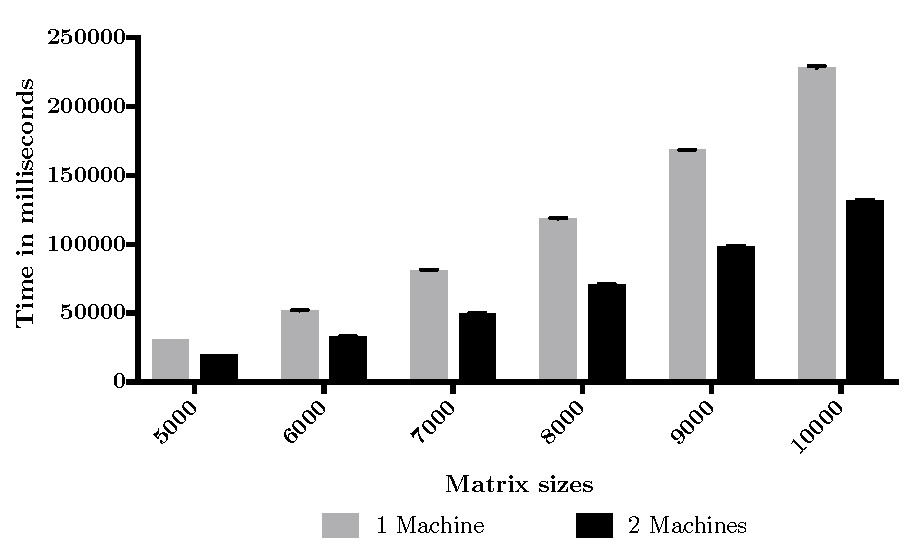
\includegraphics[width=1.0\textwidth]{images/sharded_matrix_multi.pdf}
	\centering
	\caption{Parallel Matrix Multiplication}
	\label{img:parallel_matrix}
\end{figure}

Figure \ref{img:parallel_matrix} shows that using an additional machine can lead to substantial performance benefits. It is visible that for small problem sizes the speedup is only marginal between 10-30\%. This is due to the fact that for the smaller matrix sizes the computations are executed relatively fast but are neutralized by the network interconnect that has to serve both machines at the same time. For larger matrices the ratio of computation to transferred data becomes smaller thus diminishing the network congestion effect. This can be reasoned as with rising matrix sizes of $n^2$ the computational complexity increases by $n^3$. It also becomes apparent that with growing problem sizes the speedup gets greater with a decreasing slope, which indicates that it hits a barrier around 75\%. This barrier might be imposed due to overheads by Dynamic OpenCL, Aparapi and dOpenCL but may be mainly the result of network congestions.

As matrix multiplications are computations that require noticeable amounts of data that influence the overall performance through network transfers, a second type of computation shall be evaluated that has very low data requirements. Such a workload is the Mandelbrot Set, which does not need initial data but computes values according to positions in a two dimensional array. The Mandelbrot Set was executed just as the previous matrix multiplication with 5 runs per problem size.

\begin{figure}[H]
	
	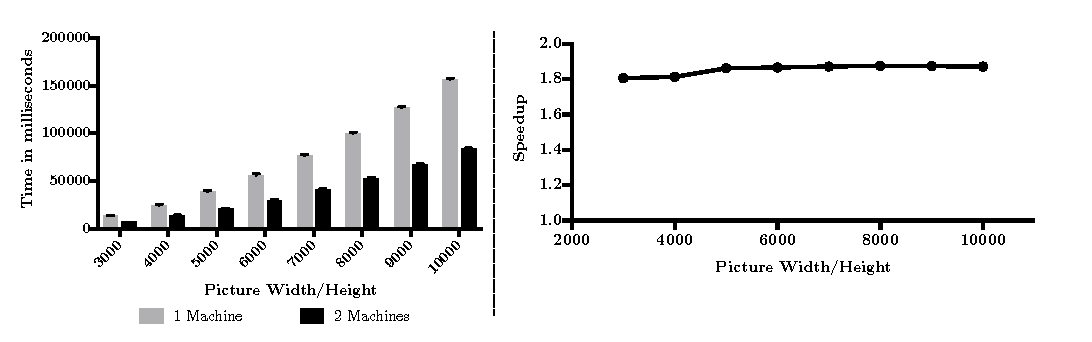
\includegraphics[width=1.0\textwidth]{images/sharded_mandelbrot.pdf}
	\centering
	\caption{Parallel Mandelbrot}
	\label{img:parallel_mandelbrot}
\end{figure}

Figure \ref{img:parallel_mandelbrot} reveals that its low data transfer requirements severely benefit the performance speedup. With speedups between 80\% and 88\% the maximum increase in performance is not only significantly higher than for the matrix multiplications but is also more stable in correlation to the problem sizes.


\subsection{Job Suite Performance}

Section \ref{single_job_performance} identified benefits when utilizing Dynamic OpenCL for a single job. In order to simulate a shared cluster environment it becomes necessary to evaluate its performance by executing variety of parallel jobs. For this reason a job suite was compiled that comprises six workloads of various complexity and type. Not only should the runtime differ per Kernel of each job but also their transferable data. The list of workloads is shown in table \ref{table:benchmark_job_setup}.

\begin{table}[!htb]
	\centering
	\begin{adjustbox}{width=0.95\textwidth}
		\small
		\begin{tabular}{l | l | l | l}
			~							& \textbf{Computational Effort}		& \textbf{Iterations}	& \textbf{Kernels per Iteration} \\
			\hline
			\textbf{Matrix Multiplication 1 (MM1)} 	& 8000x8000  								& 1 	& 5 \\
			\textbf{Matrix Multiplication 2 (MM2)}     & 6000x6000  								& 1		& 5 \\
			\textbf{Mandelbrot 1 (MB1)}     			& 1000x1000 (1000000 iterations per point) 	& 1		& 5 \\
			\textbf{Mandelbrot 2 (MB2)}     			& 2000x2000 (600000 iterations per point)  	& 1		& 5 \\
			\textbf{K-means (KM)}          			& 6000000 objects and 200 clusters  		& 10	& 1 \\
			\textbf{N-body (NB)}    		 			& 64000 objects  							& 10	& 1 \\		
		\end{tabular}
	\end{adjustbox}
	
	\caption{Benchmark Job Setup}
	\label{table:benchmark_job_setup}
\end{table}

The set of workloads thus comprises a mix of iterative and non-iterative tasks. While the iterative jobs have a fixed number of iterations and are not split per round, non-iterative tasks are split into 5 parts to enable parallelization. Although some jobs employ the same algorithm, the problem sizes are varied to create a more heterogeneous set. The implications of the problem sizes and splits for each job are explained in section \ref{workload_explanation}.

In order to prove the heterogeneity of the supplied workloads in terms of computational complexity and data transfer properties, analytical test runs are executed on a local machine of class B that measure the execution time per Kernel and the transfered data sizes. The following figure display the results of running the suite five times:

\begin{figure}[H]
	
	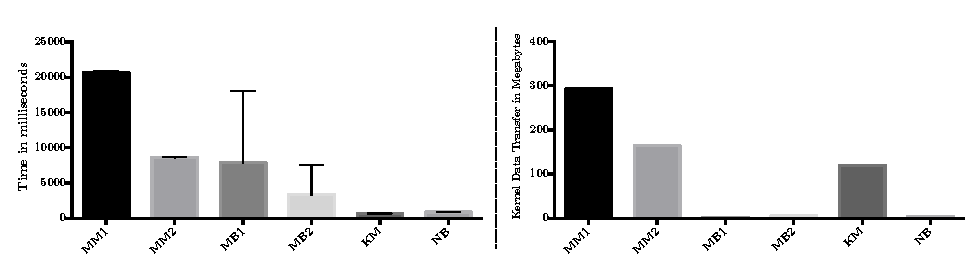
\includegraphics[width=1.0\textwidth]{images/benchmark_kernel_data_transfers.pdf}
	\centering
	\caption{Average Kernel Runtimes and Data Transfer Sizes}
	\label{img:benchmark_kernel_attributes}
\end{figure}

While it is visible that the computation times are very different, it can also be seen that the respective data transfers do not correlate to that attribute. For example, while MM2 and MB1 may require similar execution times, MM2 transfers 100x more data than MB1. The same is true for the iterative jobs KM and NB. It must be noted that MB1 and MB2 show a great standard deviation, which are not measurement errors but are a result of the nature of the algorithm. Mandelbrot calculations can not be split evenly in terms of computational effort and instead may run some Kernels for long times while having virtually no computations required by other Kernels.

For the benchmark the performance indicator to measure is the total time to finish all tasks. As the selection of scheduling algorithms has a big impact on this value, it is necessary to define the utilized algorithms. For the job scheduling tier a round robin approach is used. On the device scheduling level a historic performance based algorithm is used that assigns a Kernel to the best performing device in case multiple are available. In order to allow for a fair comparison among multiple runs, all jobs are submitted before starting the execution engine.

The suite is executed five times on three different cluster setups. At first it is executed on a single machine of class B. In this setup no network transfer is needed as the management node also executed the Kernels. For the second cluster a machine of class B is added, which is connected by a 10 Gbit/s interconnect. Therefore, some Kernels may have to be sent over the network while others will be executed directly on the management node. In the final run another machine of class A is added, which is only connected with 1 Gbit/s but has a very high computational capability. The results of the benchmark are visible in the following figure:

\begin{figure}[H]
	
	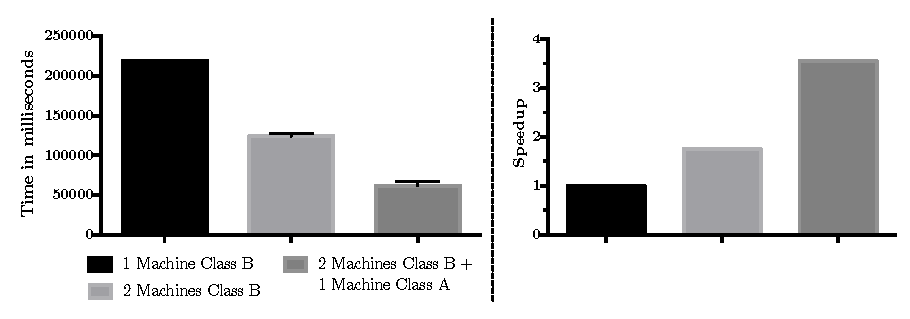
\includegraphics[width=1.0\textwidth]{images/local_full_benchmark_results.pdf}
	\centering
	\caption{Local Benchmark Results}
	\label{img:local_benchmark_results}
\end{figure}

The results indicate that employing a second machine that is connected through a fast Ethernet connection can produce significant performance benefits. Although Kernels have to be sent over the network to the second machine, it still yields an average speedup of x1.76. It also reveals that the scheduling works sufficiently even though it is based on naive algorithms. In the last cluster setup the high performance machine of class A is added, which is connected only by 1 Gbit/s. Even though the network slows down the execution times on this machine it can still double the performance of the cluster, leading to a speedup of x3.54. Thus it can be concluded that the parallelization by Dynamic OpenCL through remote machines is a viable option within a local cluster. It has to be noted though that high performance machines like machines of class A may be underutilized and slowed down by network transfers.

\section{Hybrid Distribution}


mention utilized aws region
  \chapter{Demonstration}
\label{demonstration}
In the previous chapters Dynamic OpenCL is utilized as a library, being included for single jobs or a predetermined amount of mixed workloads. Hence, it only acts on behalf of the calling code and is never used in a truly shared environment where multiple users are allowed to submit their respective workloads. Therefore this chapter showcases a developed software that allows users to compute jobs through a web interface with the option to adjust the computational capabilities during execution. For this the software is connected to the EC2 and can therefore operate a hybrid cloud. In this demonstrated use case users can not submit their own programs but can choose from a variety of already implemented algorithms that can process supplied input. For instance, users can provide data for two matrices, which shall be multiplied, although the executing algorithm is already given by the system.

\section{Architecture}

\begin{figure}[!htb]
	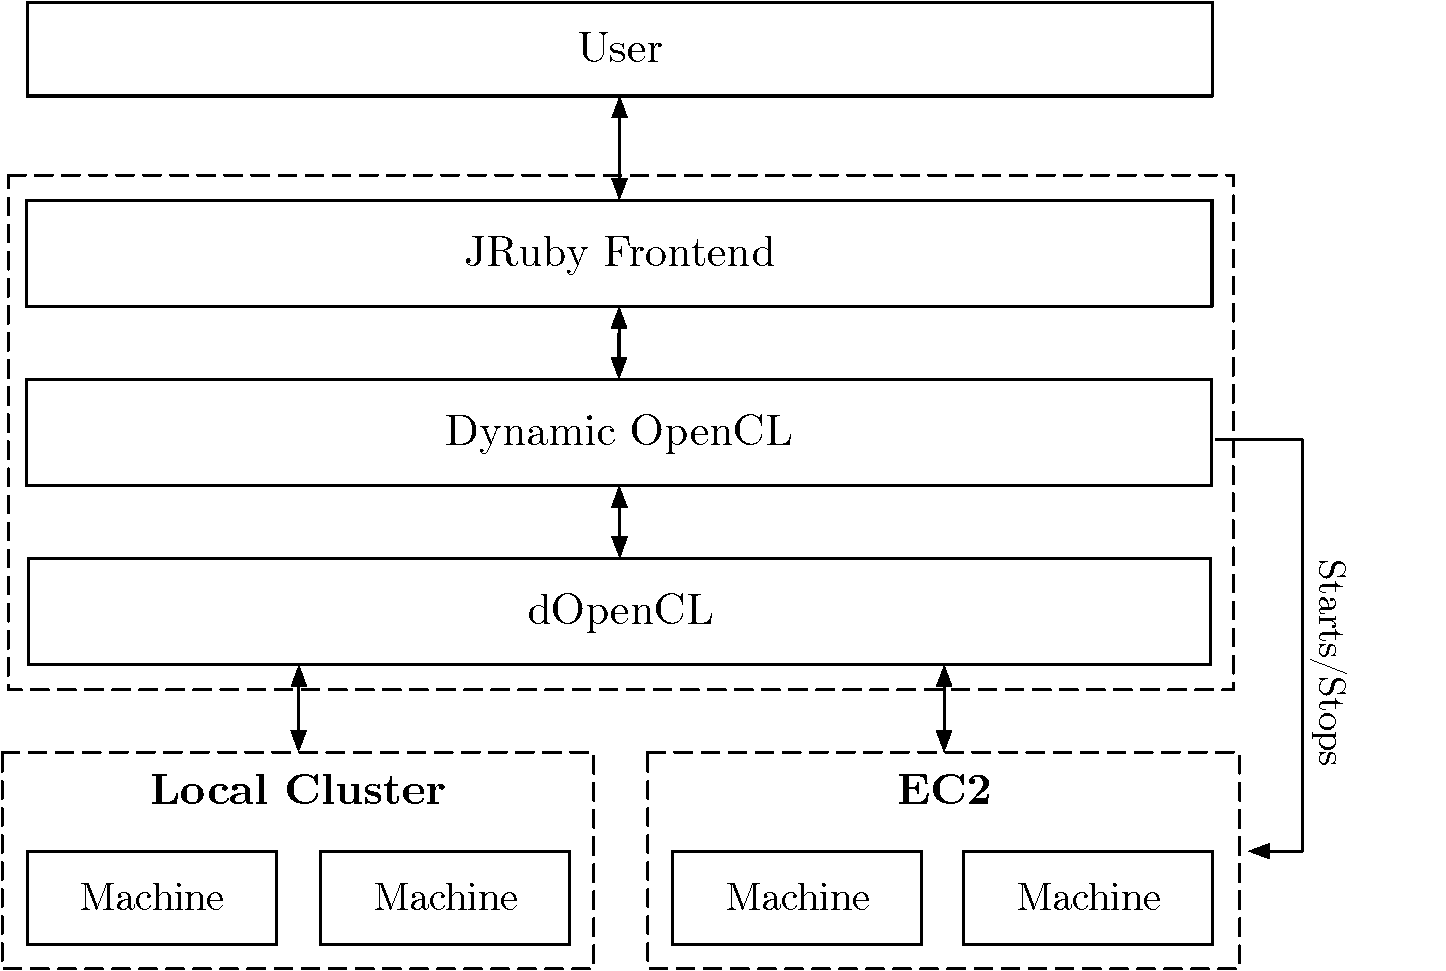
\includegraphics[width=0.7\textwidth]{drawings/demo_architecture.pdf}
	\centering
	\caption{Demo Architecture}
	\label{img:demo_architecture}
\end{figure}
The architecture of the developed system is shown in figure \ref{img:demo_architecture}. Users can access the service via a web frontend on the management node. As Dynamic OpenCL is written in Java and hence distributed as a \textit{Java Archive} file, the web frontend must run in a JVM. In this case the web server is written in Ruby and runs as a JRuby application, which executes the Ruby code in a JVM. 

The web site offers user interfaces for submitting jobs, reviewing progress and changing the cluster configuration. It mainly communicates with Dynamic OpenCL, passing execution calls to it as well as retrieving necessary information. Dynamic OpenCL then is connected to the local dOpenCL installation that carries out the actual computations either on local hardware or cloud resources. The web frontend also allows users to dynamically book cloud instances. These bookings are carried out by Dynamic OpenCL through the AWS SDK, which communicates with the EC2 cloud.
\section{User Interface}

The system gives users the possibility to manually book or disband cloud resources based on their requirements and current resource utilization. Figure \ref{img:machine_order} shows the form that provides these functions. The currently available cloud resources are listed and can be released by pressing a button in the table. This view ignores local resources as those can not be simply disbanded and therefore only lists already running cloud instances. Below the table is a drop-down list with all available EC2 instance types, which is used to specify the resources to book.

\begin{figure}[!htb]
	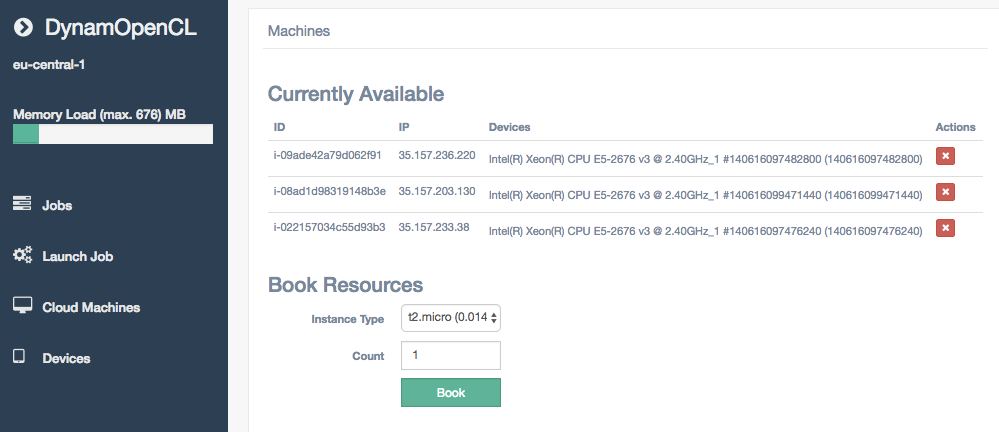
\includegraphics[width=1\textwidth]{screenshots/machine_order.png}
	\centering
	\caption{Ordering Cloud Resources}
	\label{img:machine_order}
\end{figure}

In figure \ref{img:available_devices} the device listing is portrayed that includes all devices that are available through dOpenCL. The list includes local resources as well as the cloud resources, which are accordingly marked. It also portrays the names of the devices, which includes clock speeds and number of cores. 

\begin{figure}[!htb]
	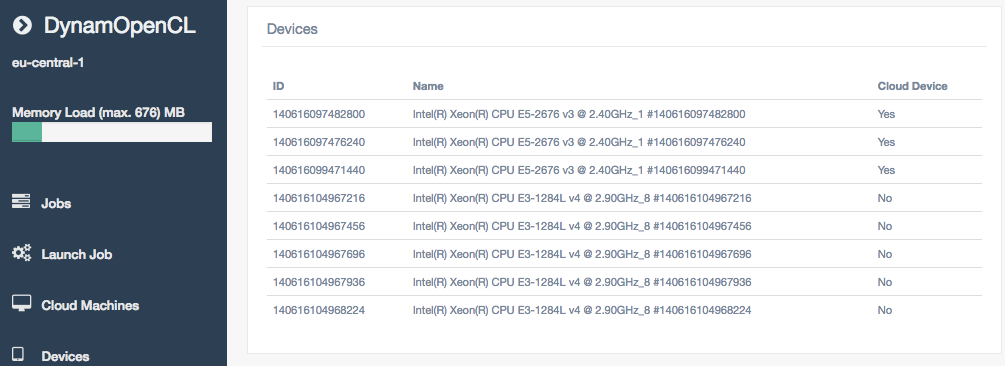
\includegraphics[width=1\textwidth]{screenshots/available_devices.png}
	\centering
	\caption{List of available Devices}
	\label{img:available_devices}
\end{figure}

Submitted jobs are listed in an overview screen that includes progress information like the number of finished parts and how many parts are currently being computed. By taking historic performance measurements an estimate for the remaining time until completion can be given. A screenshot of this view can be seen in figure \ref{img:job_overview}. Pressing the \textit{Details} button for a job leads to a more fine grained view about the historic performance of the various devices.

\begin{figure}[!htb]
	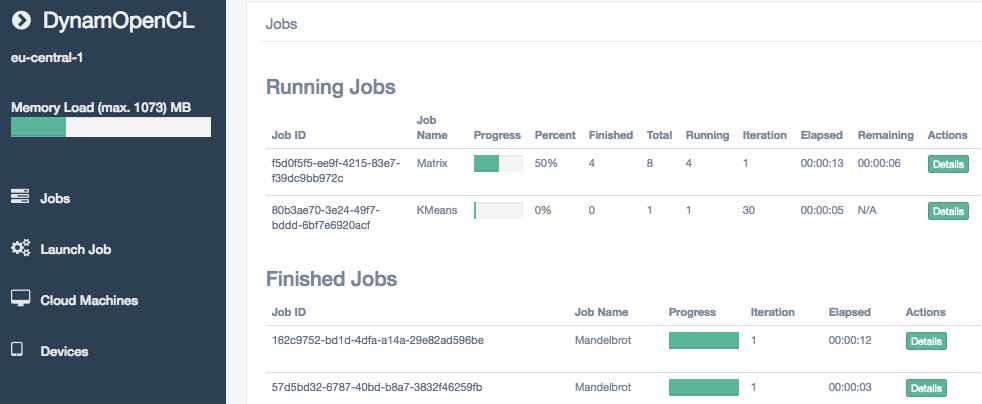
\includegraphics[width=1\textwidth]{screenshots/job_overview.png}
	\centering
	\caption{Job Overview}
	\label{img:job_overview}
\end{figure}

The details page of a job, which is displayed in figure \ref{img:job_details}, includes valuable information about the historic performance of every device that has participated in the computation of the job. It shows how many parts each device has finished as well as an average runtime per Kernel with its standard deviation. On the bottom of the page the currently active devices that compute Kernels for this job are visible.

\begin{figure}[!htb]
	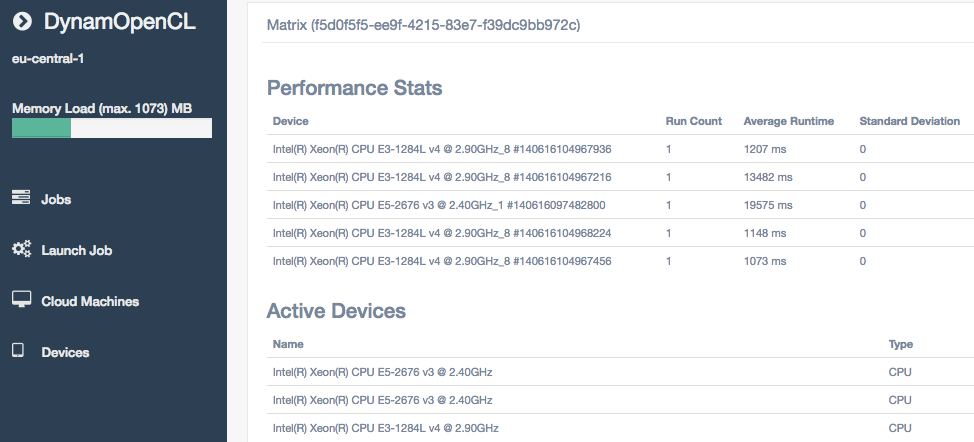
\includegraphics[width=1\textwidth]{screenshots/job_details.png}
	\centering
	\caption{Job Performance Stats}
	\label{img:job_details}
\end{figure}

	\chapter{Limitations}

Throughout this research Dynamic OpenCL is proven to efficiently compute a variety of algorithms and  execute a multitude of jobs in parallel through a two tiered scheduling infrastructure. Still, in its current version it suffers from several factors that either limit its performance or general functionality.

For instance, while Dynamic OpenCL is deeply rooted to Aparapi and profits from its compelling features it is also limited by it in the complexity of producible code. As explained in section \ref{aparapi} not every Java code can be translated to OpenCL by Aparapi and the respective capabilities of Dynamic OpenCL are therefore tied to Aparapi. Missing features might thus hinder programmers to efficiently write their code or to access low level OpenCL features. Additionally, Aparapi only supports CPUs and GPUs, thus restricting the underlying OpenCL framework that is capable of handling FPGAs and DSPs as well. There have been efforts to allow Aparapi execution on certain FPGAs but none of these modifications have been integrated in the original repository yet\cite{aparapi_ucores}.

While Dynamic OpenCL is able to operate heterogeneous clusters with different hardware vendors and device types, the varying feature sets of devices may become problematic for certain workloads. In section \ref{opencl} an example about the \textit{FP64} feature was portrayed that might be missing for some devices within a cluster. Dynamic OpenCL is currently not able to identify these features and can therefore not schedule appropriately. This means that workloads with a requirement for a specific feature may be assigned to nonsupporting devices and thus produce an error.

During the evaluation Dynamic OpenCL was run for many different cluster compositions and workloads. It is concluded that the network bandwidth is the major limiting performance factor. While this bottleneck is identifiable by the executed benchmarks, another hardware limitation exists that is caused by the architecture of Dynamic OpenCL. In the cluster setup a central node is necessary that manages all running tasks and distributes accompanying data. Throughout the execution of a job it has to hold on to input data while it also receives partial results from the compute nodes. This data has to be kept in memory and in the case of multiple data intense jobs can fill the entire memory. In an appropriate cluster setup the central node should therefore hold sufficient memory to support expected peaks in parallel running jobs. Another strategy is to block further job submissions once memory reaches a certain threshold.

\chapter{Future Work}

In its current state Dynamic OpenCL is a research prototype and therefore still requires significant improvements concerning stability. Additionally, certain features that tackle the previously described limitations of the framework are desirable in the future. While there are numerous potential improvements to the framework, this section covers more substantial topics that can greatly enhance the performance and usability of Dynamic OpenCL.

\section*{Workload Queuing}

\begin{figure}[!htb]	
	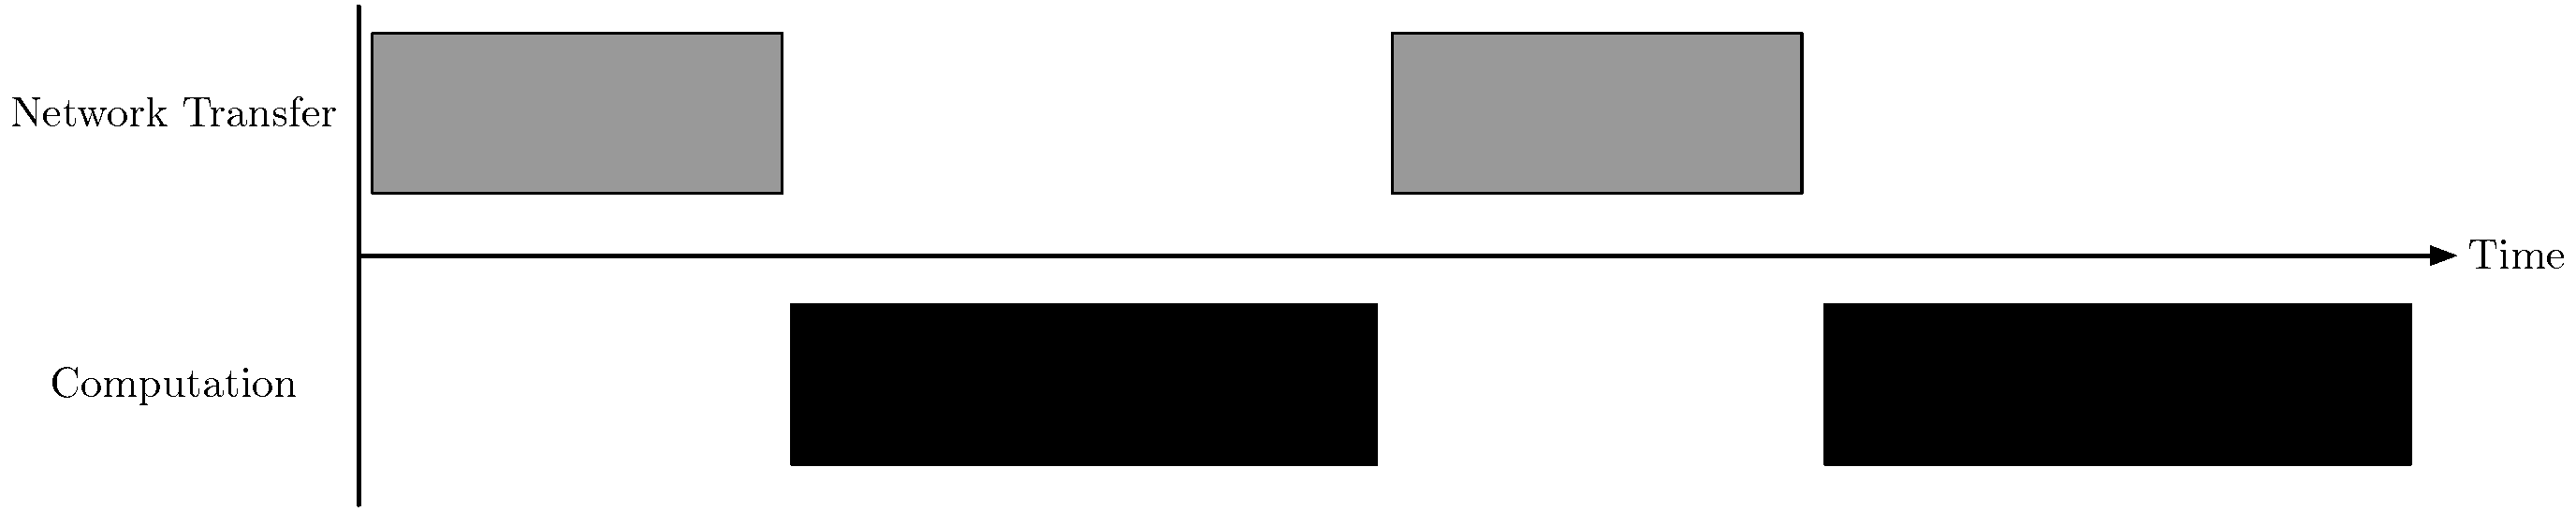
\includegraphics[width=0.85\textwidth]{drawings/missing_queue.pdf}
	\centering
	\caption{Current Execution Workflow}
	\label{img:missing_queuing}
\end{figure}
As shown by the evaluation the overall performance of Dynamic OpenCL is heavily dependent on the available networking capabilities within the cluster. In the current version there might be periods were data transfers to different machines overlap, thus competing for bandwidth. At other times when all devices in the cluster are computing, no data transfers are processed. In figure \ref{img:missing_queuing} the workflow for two subsequent tasks on a compute node is shown. Before the first task can start its data has to be transported to the compute node. As soon as the execution finishes, the output is sent back and the input for its next task is received. During the execution the network connection remains idle. One possibility to improve execution speed of the system is to reduce these idle times and instead use the available bandwidth to transfer data for future tasks. Thus, a subsequent task could start immediately once the previous workload has finished. This way these transfer times would not account to the overall runtime as they would overlap with execution phases. The envisioned workflow is displayed in figure \ref{img:active_queueing}.

\begin{figure}[!htb]	
	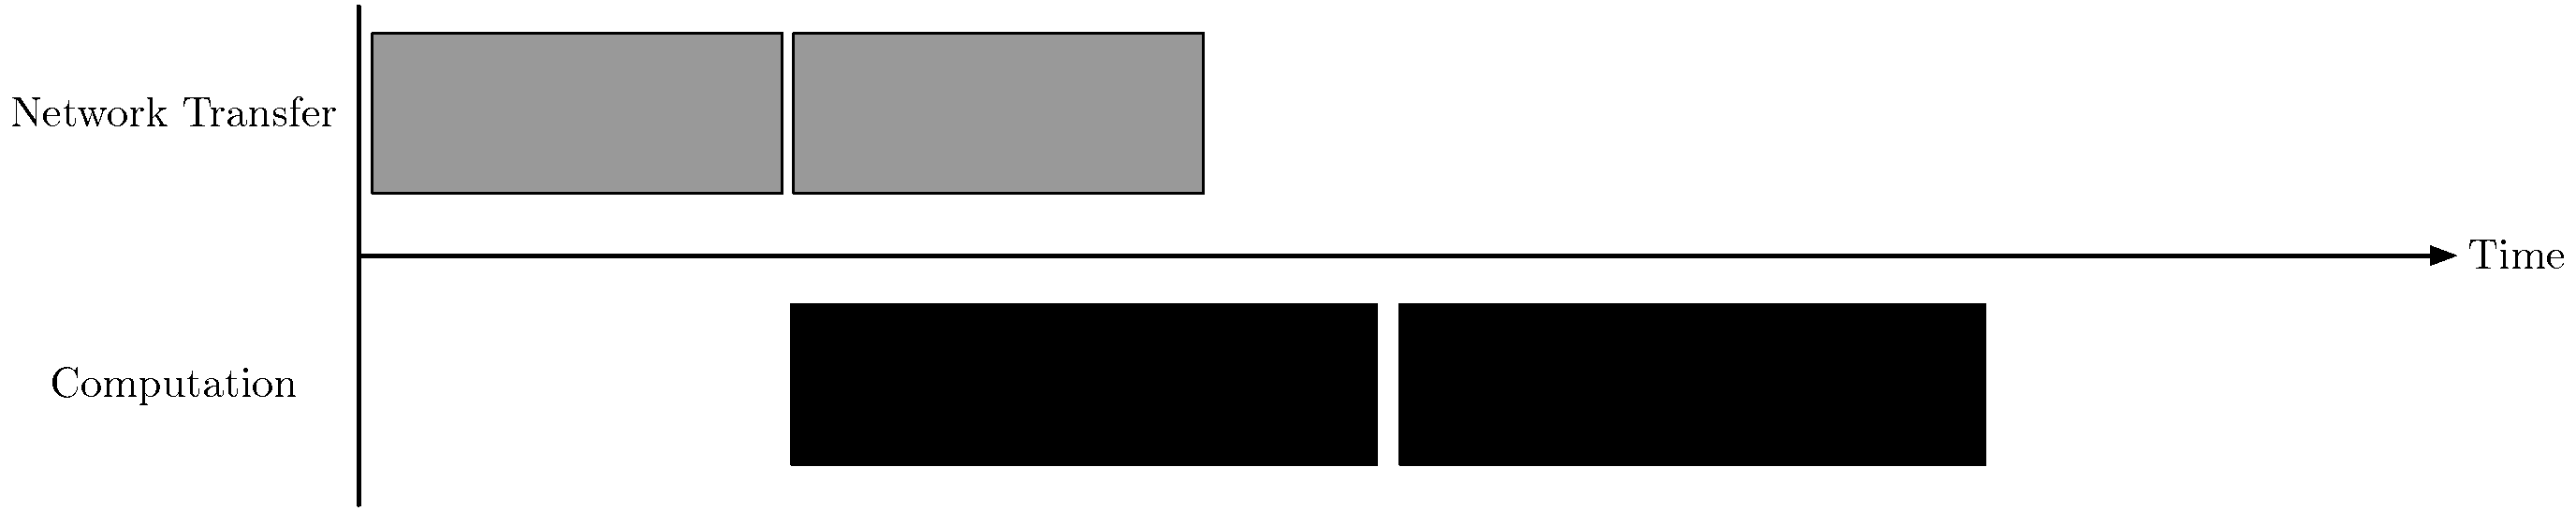
\includegraphics[width=0.85\textwidth]{drawings/active_queue.pdf}
	\centering
	\caption{Future Execution Workflow}
	\label{img:active_queueing}
\end{figure}

In the future workflow once an execution starts the input data of another task can already be transferred, thus queuing that task on the respective machine. Such a mechanism is not trivial to implement. In the given architecture dOpenCL in its current state is only forwarding OpenCL commands. This way it is possible to transfer data buffers to devices that already have another task running. Indeed this may cause memory problems as then two tasks compete for resources on the device and it must be ensured that enough memory is available for both. Instead in the future workflow tasks should be ensured to have entire control over a device without upcoming tasks interfering. It is envisioned to extend dOpenCL by a precaching mechanism that allows to send data buffers to compute nodes beforehand that are held in the main memory or serialized to disk. Once the actual buffer transfer would take place the data is already present on the compute node and only has to be sent from memory to the device.

\section*{Cloud Optimizations}

During the evaluation it was shown that Dynamic OpenCL supports hybrid clusters as well as pure cloud clusters. The prices for the various cloud resources are usually fixed rates. For example each instance type on the EC2 has an \textit{On-Demand} hourly rate that users pay to gain access to an instance for as long as they desire. 

In the current version Dynamic OpenCL supports the manual adjustment of cloud resources. A meaningful feature for users could be the automatic adjustment by the system itself based on deadlines given by the user. For example, when the user submits a job that should be executed within 8 hours, the system might identify that the current computational capabilities are insufficient to reach the deadline. Thus it might book additional cloud resources fitting the actual requirements. Additionally it could recognize certain instance types that perform exceptionally well for a given job and decide to procure more instances of this type.

Another envisioned feature is the optimization of cloud costs by utilizing dynamic pricing features if offered by the respective cloud provider. For example Amazon provides such a feature for its EC2, which is called \textit{Spot Instances}. Heavily underutilized instance types are offered to customers in auctions in which they bid a price they are willing to pay for an instance of a specified type per hour. According to Amazon when their bid is accepted they gain access to the instance for as long as they require the instance or until someone exceeds their bid and no other instances are available in the spot pool\cite{spot_instances}. It was shown by \citeauthor{spot_instance_pricing} that the bidding system is intransparent and that the price is probably not market driven but instead set by an algorithm that is based on other factors like reserve capacity\cite{spot_instance_pricing}. They assume this system is used as the number of spare instances is usually higher than the actual demand, which would result in low spot prices that are uneconomical for Amazon. 
\begin{figure}[!htb]	
	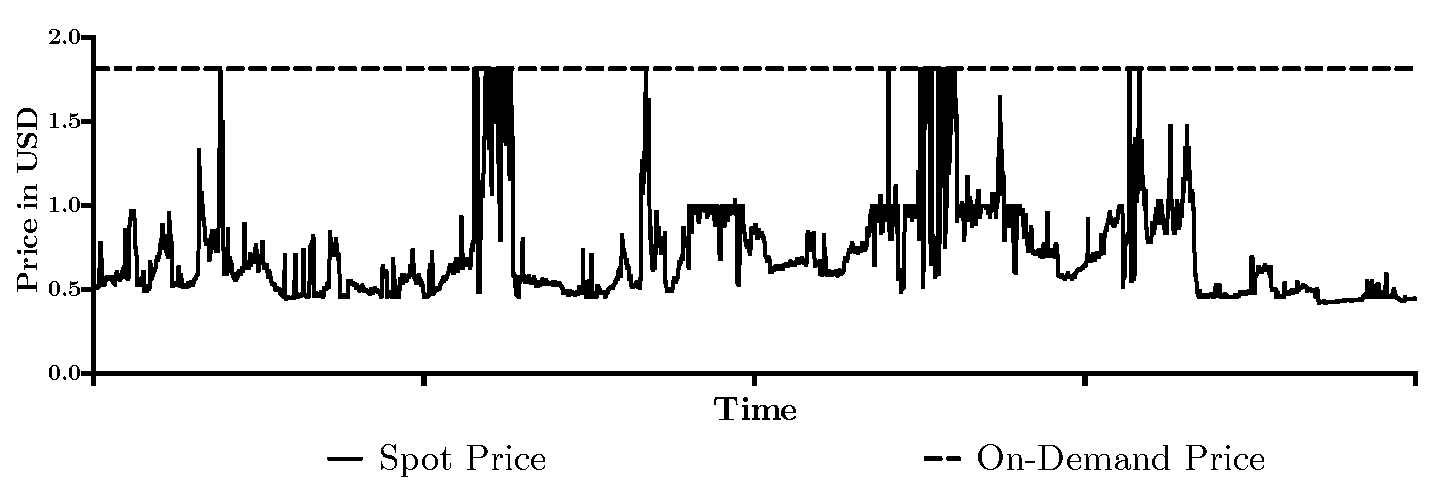
\includegraphics[width=0.7\textwidth]{images/ec2_spot_prices.pdf}
	\centering
	\caption{EC2 Spot Price Rate for c4.8xlarge Instances}
	\label{img:spot_pricing}
\end{figure}
Nevertheless spot instances offer strong discounts over on-demand prices as shown in figure \ref{img:spot_pricing}, which depicts real historic prices for a week. The on-demand price fluctuates strongly below the on-demand barrier, at times reaching values that are 23\% of the on-demand price. Utilizing historic data and knowledge about Amazon's pricing algorithm, Dynamic OpenCL could indicate users when to book spot instances for cheaper job executions or make these decisions automatically.

\chapter{Conclusion}

In this research Dynamic OpenCL is introduced, which represents a framework for distributing parallel computations among multiple machines within a cluster. Its development is based on goals defined in section \ref{goals}. Dynamic OpenCL allows to utilize \textit{heterogeneous} compute devices by employing OpenCL as its underlying computational framework. Thus, CPUs and GPUs of various vendors can be used that make it possible to efficiently process \textit{diverse workloads}. Distributing workloads across a cluster is enabled by dOpenCL, which allows to access remote devices without changes to the OpenCL code. Aparapi is added to the framework in order to allow users an \textit{ease of programming} by writing OpenCL Kernels in Java. Additionally Dynamic OpenCL introduces its own execution model in which computations are split into partials, which can be executed in parallel on multiple devices. Dynamic OpenCL also allows to dynamically \textit{scale resources} by adding cloud resources to the cluster. An extendable scheduling architecture is utilized for \textit{scaling execution speeds} of jobs. Different scheduling algorithms also allows to adapt to complex cluster setups like hybrid clusters in order to provide an \textit{optimized scheduling} solution.

The extensive evaluation shows that Dynamic OpenCL is able to operate various cluster setups and allows efficient execution for mixed workloads. In all portrayed environments the framework yields significant improvements to performance when employing additional machines. It is shown that the individual achievable speedups are dependent on the data intensity of the respective workloads as well as the available network bandwidths. Even in a heavily bottlenecked scenario of a hybrid cluster, remote cloud resources can assist computations noticeably when employing a suitable scheduling strategy. Aside from pure performance considerations, Dynamic OpenCL also enables cluster administrators to reach better hardware utilization by dynamic resource adjustments. This may lead to individual monetary benefits by reducing the total cost of ownership for hardware.

Overall Dynamic OpenCL allows users access to distributed cluster computations at a high abstraction level. Not only does it offer inexperienced users to overcome the steep learning curve of OpenCL but also aids seasoned programmers to develop their programs faster by eliminating OpenCL boilerplate code. In order to harness parallel compute resources, programmers may split their datasets manually into partials, which is deemed to be intuitive in an object oriented environment like Java. 

Dynamic OpenCL is conceived with adaptability in mind regarding cloud services. As such it can be adjusted to new upcoming cloud providers with minor changes. Additionally, cloud provides like Amazon are currently introducing novel resource types like FPGAs\cite{amazon_fpga}. Utilizing these devices is possible by the underlying OpenCL model but is currently not supported by Aparapi. Thus, harnessing these powerful devices still requires additional work to Dynamic OpenCL.



	% Bibliographie
	\addcontentsline{toc}{chapter}{\refname}
	\printbibliography


	% ggf. Anhang
	\appendix\thispagestyle{empty}
\begin{center}\textsf{\textbf{Zusammenfassung}}\end{center}

\noindent Eine zentrale Herausforderung der Softwareentwicklung stellt die Parallelisierung von Algorithmen aus Gründen der Performancesteigerung dar. Das Erzeugen von parallelen Programmen erfordert tiefgründige Kenntnis der verfügbaren Hardwarearchitekturen und nutzbaren Programmiermodelle. Um eine gehobene Form der Parallelisierung zu erreichen, ist es außerdem notwendig, Programme mit Multi-Core-Unterstützung auf mehrere Maschinen innerhalb eines Clusters zu verteilen. Dieser Schritt führt zu einem erhöhten Kommunikationsaufwand, der die Komplexität der jeweiligen Algorithmen erhöht. Das Forschungsziel dieser Arbeit ist die Schaffung eines Frameworks zur Verteilung von parallelen Berechnungen auf CPUs und GPUs innerhalb eines Clusters, welches seine Funktionalität über eine API auf hoher Abstraktionsebene bereitstellt. Somit sollen Nutzer ermächtigt werden, ohne detaillierte Fachkenntnis verteilte parallele Programme zu erstellen. Als weiteres Hauptmerkmal soll es möglich sein, die Ressourcen eines Clusters dynamisch an die benötigten Rechenkapazitäten anzupassen.

Aufgrund der Vielzahl an verfügbaren Parallelisierungsmethoden wie OpenMP, MPI und OpenCL ist es notwendig, das jeweilige Nutzungspotenzial für das Framework zu bestimmen. Da OpenCL es ermöglicht, portable parallele Programme über ein festes Programmiermodell zu erzeugen, wird es als zentrale Technologie des Frameworks ausgewählt. In Kombination mit dOpenCL können OpenCL Programme ohne Änderungen des Programmcodes auf entfernten Maschinen ausgeführt werden. Das daraus resultierende Parallelisierungspotenzial wird innerhalb des implementierten Frameworks, genannt Dynamic OpenCL, abstrahiert. Es stellt somit den zentralen Beitrag dieser Forschung dar. Dynamic OpenCL ist in Java verfasst und ermöglicht es Programmierern, verteilte OpenCL Programme in Java zu erzeugen. Durch Mechanismen zur Verwaltung individueller Clusterstrukturen und über die Möglichkeit der dynamischen Anpassung der verwendeten Ressourcen kann Dynamic OpenCL in unterschiedlichen Anwendungsfällen eingesetzt werden.

Während der ausführlichen Evaluierung von Dynamic OpenCL kann gezeigt werden, dass erhebliche Performancesteigerungen durch die Parallelisierung möglich sind. Auch in komplexen Clusterstrukturen mit angebundenen Cloudressourcen können Ausführungszeiten mit Hilfe von spezialisierten Scheduling-Algorithmen signifikant verringert werden. Auf der Basis von Dynamic OpenCL wird ein prototypischer Web-Server präsentiert, der Nutzern die Ausführung von vorgefertigten Algorithmen über ein grafische Oberfläche ermöglicht. Die Oberfläche erlaubt es ebenfalls, die Rechenkapazität des Clusters dynamisch nach Belieben anzupassen.

Es wird aufgezeigt, dass Dynamic OpenCL in der Lage ist, in unterschiedlichen Umgebungen deutliche Leistungssteigerungen herbeizuführen. Dabei ist das Potenzial der Verbesserung größtenteils abhängig vom jeweiligen Algorithmus und der verfügbaren Netzwerkbandbreite des Clusters. Durch zukünftige Verbesserungen an Dynamic OpenCL, die Engpässe bei der Verteilung von Aufgaben über das Netzwerk umgehen, können weitere Beschleunigungen in Aussicht gestellt werden.
	\appendix\chapter{\appendixname}

\section{Eins}
Lorem ipsum dolor sit amet, consetetur sadipscing elitr, sed diam nonumy eirmod tempor invidunt ut labore et dolore magna aliquyam erat, sed diam voluptua. At vero eos et accusam et justo duo dolores et ea rebum.

\section{Zwei}
Stet clita kasd gubergren, no sea takimata sanctus est Lorem ipsum dolor sit amet. Lorem ipsum dolor sit amet, consetetur sadipscing elitr, sed diam nonumy eirmod tempor invidunt ut labore et dolore magna aliquyam erat, sed diam voluptua. 

\section{Drei}
At vero eos et accusam et justo duo dolores et ea rebum. Stet clita kasd gubergren, no sea takimata sanctus est Lorem ipsum dolor sit amet. % example

	% Eigenständigkeitserklärung
	\ifisbook\pagestyle{plain}\cleardoubleemptypage%\addchap{Eidesstattliche Erklärung}
\begin{center}\textsf{\textbf{Eidesstattliche Erklärung}}\end{center}
Hiermit versichere ich, dass meine {\hpitype} \enquote{\hpititle} (\enquote{\hpititleother}) selbständig verfasst wurde und dass keine anderen Quellen und Hilfsmittel als die angegebenen benutzt wurden. Diese Aussage trifft auch für alle Implementierungen und Dokumentationen im Rahmen dieses Projektes zu.\\

% <= Laut Aussage des Studienreferats braucht es - auch wenn die Arbeit in englischer Sprache verfasst ist - KEINE separate Version der Eigenständigkeitserklärung auf Englisch. Sowohl für Arbeiten in deutscher Sprache als auch für Arbeiten in englischer Sprache genügt EINE EINZIGE Eigenständigkeitserklärung auf DEUTSCH.

\noindent
Potsdam, den \hpidate,
\vspace{2cm}

\begin{center}
\begin{tabular}{C{6cm}}
\hline
{\small({\hpiauthor})}
\end{tabular}
\end{center}

\fi

\end{document}
